\documentclass{fenicscourse}
% General math notation
\newcommand{\N}{\mathbb{N}}
\newcommand{\PP}{\mathbb{P}}
\newcommand{\QQ}{\mathbb{Q}}

% Math operators
\DeclareMathOperator{\ord}{ord}
\DeclareMathOperator{\Kern}{ker}
\DeclareMathOperator{\Image}{im}
\DeclareMathOperator{\spann}{span}
\DeclareMathOperator{\diam}{diam}


% Mesh and FEM notation
%\newcommand{\dx}{\, \mathrm{d} x}
%\newcommand{\ds}{\, \mathrm{d} s}
%\newcommand{\dS}{\, \mathrm{d} S}
\newcommand{\mesh}{\mathcal{T}}
\newcommand{\facets}{\mathcal{F}}
\newcommand{\inmesh}{\partial_i \mathcal{T}}
\newcommand{\exmesh}{\partial_e \mathcal{T}}

\newcommand{\jump}[1]{\llbracket #1 \rrbracket}
\newcommand{\avg}[1]{\langle #1 \rangle}
\newcommand{\meanvalue}[1]{\langle #1 \rangle}
\newcommand{\vect}[1]{\mathbf{#1}}

\newcommand{\gradhterm}[2]{(\nabla_h #1, \nabla_h #2)_{\Omega}}
\newcommand{\consterm}[2]{(\avg{\nabla_h #1} \dotn,\jump{#2})_{\inmesh}}
\newcommand{\penterm}[2]{( h^{-1} \jump{#1}, \jump{#2})_{\inmesh}}

\newcommand{\Ctr}{C_{\text{tr}}}

% Abbreviations for names etc
\newcommand{\apriori}{\emph{a~priori}}
\newcommand{\aposteriori}{\emph{a~posteriori}}

% Dimensions
\newcommand{\codesize}{\footnotesize}

% Environments
\DefineVerbatimEnvironment{code}{Verbatim}{frame=single,rulecolor=\color{blue}}

% Notes
\newcommand{\amnote}[1]{\todo[inline,color=blue!40]{\underline{AM:} #1}}
\newcommand{\mglnote}[1]{\todo[inline,color=red!40]{\underline{MGL:} #1}}
\newcommand{\alnote}[1]{\todo[inline,color=green!40]{\underline{AL:} #1}}
\newcommand{\mernote}[1]{\todo[inline,color=pink!40]{\underline{MER:} #1}}

% Special notation PI
\newcommand{\OmegaD}{\Omega_{0,\mathrm{D}}}
\newcommand{\OmegaN}{\Omega_{0,\mathrm{N}}}
\newcommand{\OmegaO}{\Omega_{_\mathrm{O}}}
\newcommand{\bfsigma}{{\pmb\sigma}}
\newcommand{\bfepsilon}{{\pmb\epsilon}}

% Special notation for PII
\newcommand{\bfu}{\boldsymbol{u}}
\newcommand{\bff}{\boldsymbol{f}}
\newcommand{\bfg}{\boldsymbol{g}}
\newcommand{\bfv}{\boldsymbol{v}}
\newcommand{\bfe}{\boldsymbol{e}}
\newcommand{\bfn}{\boldsymbol{n}}
\newcommand{\bfx}{\boldsymbol{x}}
\newcommand{\Oast}{\Omega^{\ast}}
\newcommand{\Vast}{\mathcal{V}^{\ast}}

%\newcommand{\meshast}{\mathcal{T}_{\ast}}
\newcommand{\pO}{\partial \Omega}
\newcommand{\meshast}{\mathcal{T}^{\ast}}
\newcommand{\Fast}{\mathcal{F}^{\ast}_{\Gamma}}
\newcommand{\piast}{\pi^{\ast}_h}
\newcommand{\tnast}{\tn_{\ast}}
\newcommand{\tnsip}{\tn_{\text{sip}}}
\newcommand{\tnsipast}{\tn_{\text{sip},\ast}}
\newcommand{\asip}{a^{\text{sip}}_h}

\newcommand{\mcF}{\mathcal{F}}
\newcommand{\mcT}{\mathcal{T}}
\newcommand{\mcV}{\mathcal{V}}
\newcommand{\mcE}{\mathcal{E}}
\newcommand{\mcN}{\mathcal{N}}
\newcommand{\mcC}{\mathcal{C}}
\newcommand{\mcA}{\mathcal{A}}
\newcommand{\tn}{|\mspace{-1mu}|\mspace{-1mu}|}
\newcommand{\Pzero}{P_h^{0,\mathrm{dc}}}
\newcommand{\Pone}{P_h^1}
\newcommand{\ndot}{\bfn \cdot}
\newcommand{\dotn}{\cdot \bfn}
\newcommand{\bfw}{\boldsymbol{w}}
\newcommand{\Wspace}{{\mathcal{V}_h}}

% Special notation for PIII
\newcommand{\nablan}{\partial_{\bfn}}
\newcommand{\OmcupOm}{\Omega_1 \cup \Omega_2}
\newcommand{\mcupm}{{\mathcal{T}^{\ast}_1} \cup \mesh_2}
%\newcommand{\mcupm}{{\meshast}_1 \cup \mesh_2}
%\newcommand{\meanvalue}[1]{\langle #1 \rangle_{\alpha}}
\newcommand{\ifnormalpha}[1]{\ifnorm{#1}{\alpha}}
\newcommand{\ifnorm}[2]{\| #1 \|_{#2,h,\Gamma}}
\newcommand{\tildev}{\widetilde{\bfv}}
\newcommand{\bfphi}{\boldsymbol{\phi}}
\newcommand{\picorr}{\pi^c}

% Math macros
\newcommand{\renni}[2]{\langle #2 ,\; #1 \rangle}


\begin{document}

\fenicslecture{Lecture 23: Biot's equations of poroelasticity}
              {Kent-Andre Mardal}


\begin{frame}
\frametitle{Biot's equations of poroelasticity} 
The Biot's equations of poroelasticity describe the fluid--structure interaction
between a porous elastic media saturated  
by a pressurized fluid 

\vspace{0.3cm}
The equations have many forms, one common form is the displacement-pressure formulation: 
\begin{eqnarray*}
\rho u_{tt} - \nabla\cdot 2 \mu \epsilon(u) - \nabla \lambda \nabla \cdot u I + \alpha \nabla p &=& f \\   
s \frac{\partial p}{\partial t} + \alpha \frac{\nabla \cdot u}{\partial t} - \nabla \cdot (K \nabla p) &=& g 
\end{eqnarray*}
Here 
\begin{itemize}
\item $u$ and $p$ are the uknown displacement and pressure
\item $\rho$ is the density 
\item $\mu$ and $\lambda$ are  Lam\'{e}'s elastic parameters
\item $s$ is the storage coefficent
\item $K$ is the hydralic conductivity (permeability / viscosity) 
\end{itemize}
\emph{The challenge is to find schemes that are robust to (large) variations
in particular in $\lambda$ and $K$.} 
\end{frame}

\begin{frame}
\frametitle{Biot's equations of poroelasticity} 
The equations are a coupling of linear elasticity 
and porous Darcy flow. It has a number of
intesting and challenging features: 
\begin{enumerate}
\item Second order derivative in time  
$\rho u_{tt}$ 
\item First order derivatives in time 
$ s \frac{\partial p}{\partial t}$ and $ \alpha \frac{\nabla \cdot u}{\partial t}$
\item Three elliptic terms 
$\nabla\cdot 2 \mu \epsilon(u)$, $\nabla \lambda \nabla \cdot u I$, and  $\nabla \cdot (K \nabla p)$ 
\item 
$\nabla \lambda \nabla \cdot u I$ is associated with locking of the displacement as we learned 
in linear elasticity  
\item For $\nabla \cdot (K \nabla p)$, $K$ may be very small or contain large discontinuities resulting in
pressure oscillations  
\end{enumerate}
Hence, this is a challenging numerical problem which is currently heavily investigated
\end{frame}

\begin{frame}
\frametitle{Biot's equations of poroelasticity} 
In the quasi-static formulation we ignore the term 
$\rho u_{tt}$. This can be done as long as the application 
in focus does not involve shear or compression waves.  
\vspace{0.3cm}
The equation can the be written:  
\begin{eqnarray*}
 \nabla\cdot 2 \mu \epsilon(u) - \nabla \lambda \nabla \cdot u I + \nabla p &=& f \\   
s \frac{\partial p}{\partial t} + \alpha \frac{\nabla \cdot u}{\partial t} - \nabla \cdot (K \nabla p) &=& g 
\end{eqnarray*}

\end{frame}

\begin{frame}
\frametitle{Variational formulation}
\begin{eqnarray}
\label{mom}
 \nabla\cdot 2 \mu \epsilon(u) - \nabla \lambda \nabla \cdot u I + \nabla p &=& f \\   
\label{cont}
s \frac{\partial p}{\partial t} + \alpha \frac{\nabla \cdot u}{\partial t} - \nabla \cdot (K \nabla p) &=& g 
\end{eqnarray}

We obtain a variational formulation by multiplying the momentum equation, \eqref{mom}, by $v$ and integrating by parts
\[ 
\int_\Omega 2 \mu \epsilon(u) : \epsilon(v) \dx + 
\int_\Omega \lambda  \nabla \cdot u \nabla \cdot v \dx -
\int_\Omega p \nabla \cdot v \dx = 
\int_\Omega f v \dx 
\]
Similarly, multiplying the continuity equation, \eqref{cont}, by $q$ and integrating by parts we obtain 
and multiplying by -1 to obtain symmetry we get 
\[
-\int_\Omega s \frac{\partial p}{\partial t} q \dx - 
\int_\Omega \alpha \frac{\nabla \cdot u}{\partial t} q \dx - 
\int_\Omega K \nabla p \cdot \nabla q \dx = 
\int_\Omega g q \dx 
\]

\end{frame}



\begin{frame}
\frametitle{Variational formulation, cont'd}
The equations 
\begin{eqnarray*} 
\int_\Omega 2 \mu \epsilon(u) : \epsilon(v) \dx + 
\int_\Omega \lambda  \nabla \cdot u \nabla \cdot v \dx -
\int_\Omega p \nabla \cdot v \dx = 
\int_\Omega f v \dx \\  
-\int_\Omega s \frac{\partial p}{\partial t} q \dx - 
\int_\Omega \alpha \frac{\nabla \cdot u}{\partial t} q \dx - 
\int_\Omega K \nabla p \cdot \nabla q \dx = 
\int_\Omega g q \dx 
\end{eqnarray*}
with an implicit Euler discretization (where we have multiplied the continuity equation 
with $\Delta t$) reads: 
The equations 
\begin{eqnarray*} 
\int_\Omega 2 \mu \epsilon(u^n) : \epsilon(v)  + 
\lambda  \nabla \cdot u^n \nabla \cdot v  -
p^n \nabla \cdot v \dx  &=& 
\int_\Omega f v  \dx \\  
\int_\Omega -s p^n q  - 
 \alpha \nabla \cdot u^n q  - 
 \Delta t K \nabla p^n \cdot \nabla q \dx &=& 
\int_\Omega \ldots \dx  
\end{eqnarray*}
\end{frame}

\begin{frame}
\frametitle{Variational formulation}
This equation may be written as a saddle point problem 
\begin{equation}
\label{biotmat}
\left[
\begin{array}{cc}
A & B \\
B^T & -C
\end{array}
\right]
\left[
\begin{array}{c} u \\ p \end{array} 
\right]
= 
\left[
\begin{array}{c} f \\ g \end{array} 
\right]
\end{equation}
Where, if $N_i$ are the basis functions for the displacement 
and $L_i$ are the basis functions of the pressure
\begin{itemize}
\item $A_{ij} =  \int_\Omega 2 \mu \epsilon(N_i) : \epsilon(N_j) \dx + \lambda  \nabla \cdot N_i \nabla \cdot N_j \dx$ 
\item $B_{ij} =  \int_\Omega  \nabla \cdot N_i L_j\dx$ 
\item $C_{ij} =  \int_\Omega s  L_i L_j \dx + K \nabla L_i \cdot \nabla L_j \dx $ 
\end{itemize}

Notice that the $C$ matrix (as $A$) is positive, but 
in \eqref{biotmat} there is a '-' sign in front of $C$. 
As for the previously mentioned mixed form of 
elasticity (with "solid pressure"), this negative term is stabilizing
the saddle point problem. 

\end{frame}

\begin{frame}
\frametitle{Comparison with Stokes}
We remember Stokes problem 
This equation may be written as a saddle point problem 
\[
\left[
\begin{array}{cc}
-\nabla^2 & -\nabla \\
\nabla\cdot & 0  
\end{array}
\right]
\left[
\begin{array}{c} u \\ p \end{array} 
\right]
= 
\left[
\begin{array}{c} f \\ 0 \end{array} 
\right]
\]

In our case $A$ and $C$ are different. 
This equation may be written as a saddle point problem 
\[
\left[
\begin{array}{cc}
-\nabla\cdot 2 \mu \epsilon - \nabla \lambda \nabla \cdot & -\nabla  \\
\nabla\cdot  & -s+\nabla\cdot K \nabla  
\end{array}
\right]
\left[
\begin{array}{c} u \\ p \end{array} 
\right]
= 
\left[
\begin{array}{c} f \\ g \end{array} 
\right]
\]

\begin{itemize}
\item We already addressed the difference between $\nabla^2$ and $\nabla\cdot \epsilon$   
\item We therefore replace $\nabla\cdot \epsilon$ with $\nabla^2$ to simplify the discussion  
\item We known that large $\lambda$ is associated with  locking of displacement  
\item Pressure oscillations are associated with  $K$ small or with large jumps  
\end{itemize}



\end{frame}

\begin{frame}
\frametitle{An attempt to avoid displacement locking: introduce solid pressure}
We remember that for linear elasticity (when $\lambda \gg \mu$) we 
introduced the solid pressure. The displacement formulation
of linear elasticity was:  
\[
-\mu \nabla^2 u  - \nabla \lambda \nabla \cdot u = f  
\]
introducing the solid pressure as $p_S = \lambda \nabla \cdot u$ we obtain 
\begin{eqnarray*}
-\mu \nabla^2 u  - \nabla p_S &=& f \\  
\nabla\cdot u - \frac{1}{\lambda} p_S &=& g 
\end{eqnarray*}
This formulation did not suffer from locking when using Brezzi stable elements such as, e.g.,
Taylor--Hood. 
\end{frame}


\begin{frame}
\frametitle{Biot with solid pressure}
Using the same trick we obtain an alternative formulation of
the Biot's equations with two pressures (solid $p_S$ and fluid $p_F$)
\[
\left[
\begin{array}{ccc}
-\nabla^2 & -\nabla & -\nabla \\
\nabla\cdot & -\frac{1}{\lambda} & 0  \\ 
\nabla\cdot & 0 &  -s + \nabla\cdot K \nabla   
\end{array}
\right]
\left[
\begin{array}{c} u \\ p_S \\ p_F \end{array} 
\right]
= 
\left[
\begin{array}{c} f \\ 0 \\ g \end{array} 
\right]
\]
\alert{Is this formulation ok?} 
\end{frame}

\begin{frame}
\frametitle{Biot with solid pressure}
Using the same trick we obtain an alternative formulation of
the Biot's equations with two pressures (solid $p_S$ and fluid $p_F$)
\[
\left[
\begin{array}{ccc}
-\nabla^2 & -\nabla & -\nabla \\
\nabla\cdot & -\frac{1}{\lambda} & 0  \\ 
\nabla\cdot & 0 &  -s + \nabla\cdot K \nabla   
\end{array}
\right]
\left[
\begin{array}{c} u \\ p_S \\ p_F \end{array} 
\right]
= 
\left[
\begin{array}{c} f \\ 0 \\ g \end{array} 
\right]
\]
As $\lambda\rightarrow\infty$ and
$K,s \rightarrow 0$ we obtain
\[
\left[
\begin{array}{ccc}
-\nabla^2 & -\nabla & -\nabla \\
\nabla\cdot & 0 & 0  \\ 
\nabla\cdot & 0 &  0   
\end{array}
\right]
\left[
\begin{array}{c} u \\ p_S \\ p_F \end{array} 
\right]
= 
\left[
\begin{array}{c} f \\ 0 \\ g \end{array} 
\right]
\]
This formulation is not stable in the parameters $\lambda$, $s$ and $K$! 


\end{frame}

\begin{frame}
\frametitle{Biot with \alert{Total} pressure}
Let us instead introduce 
the \alert{total pressure:} $p_T=p_S + p_F$. 
The problem then reads
\[
\left[
\begin{array}{ccc}
-\nabla^2 & -\nabla & 0 \\
\nabla\cdot & -\frac{1}{\lambda} & \frac{1}{\lambda}  \\ 
0 & \frac{1}{\lambda} &  -s - \frac{1}{\lambda} + \nabla\cdot K \nabla   
\end{array}
\right]
\left[
\begin{array}{c} u \\ p_S \\ p_F \end{array} 
\right]
= 
\left[
\begin{array}{c} f \\ 0 \\ g \end{array} 
\right]
\]
This formulation is perfectly stable in the parameters $\lambda$, $s$ and $K$! 

\vspace{0.3cm}
Standard Stokes elements can be used!

\vspace{0.3cm}
\footnotesize{
Lee JJ, Mardal KA, Winther R. Parameter-robust discretization and preconditioning of Biot's consolidation model. SIAM Journal on Scientific Computing. 2017 Jan 3;39(1):A1-24.
}
\end{frame}

\begin{frame}
\frametitle{The Galerkin method and oscillations}
Consider the following simplified problem in 1D 
\[
s \frac{\partial p}{\partial t} - \nabla \cdot (K \nabla p) = f 
\]
Given a small $K$, does a usual finite element scheme yield a good approximation? 
\end{frame}

\begin{frame}
\frametitle{The Galerkin method and oscillations}
An implicit Euler leads to  
\[
s p^n - \Delta t \nabla \cdot (K \nabla p^n) = p^{n-1} + \Delta t f   
\]
Given a small $K$, does a usual finite element scheme yield a good approximation? 
\end{frame}

\begin{frame}[fragile]
\frametitle{The Galerkin method and oscillations, cont'd}
\begin{python}
from dolfin import *
mesh = UnitIntervalMesh(10)
V = FunctionSpace(mesh, "Lagrange", 1) 
u = TrialFunction(V)
v = TestFunction(V)

K = Constant(0.00001)
a = u*v*dx + K*inner(grad(u), grad(v))*dx 
L = Constant(0)*v*dx 

def boundary(x): return near(x[0], 0) or near(x[0], 1) 
bc = DirichletBC(V, Constant(1), boundary)

u = Function(V)
solve(a == L, u, bc)
\end{python}
\end{frame}

\begin{frame}
\frametitle{The Galerkin method and oscillations, cont'd}
 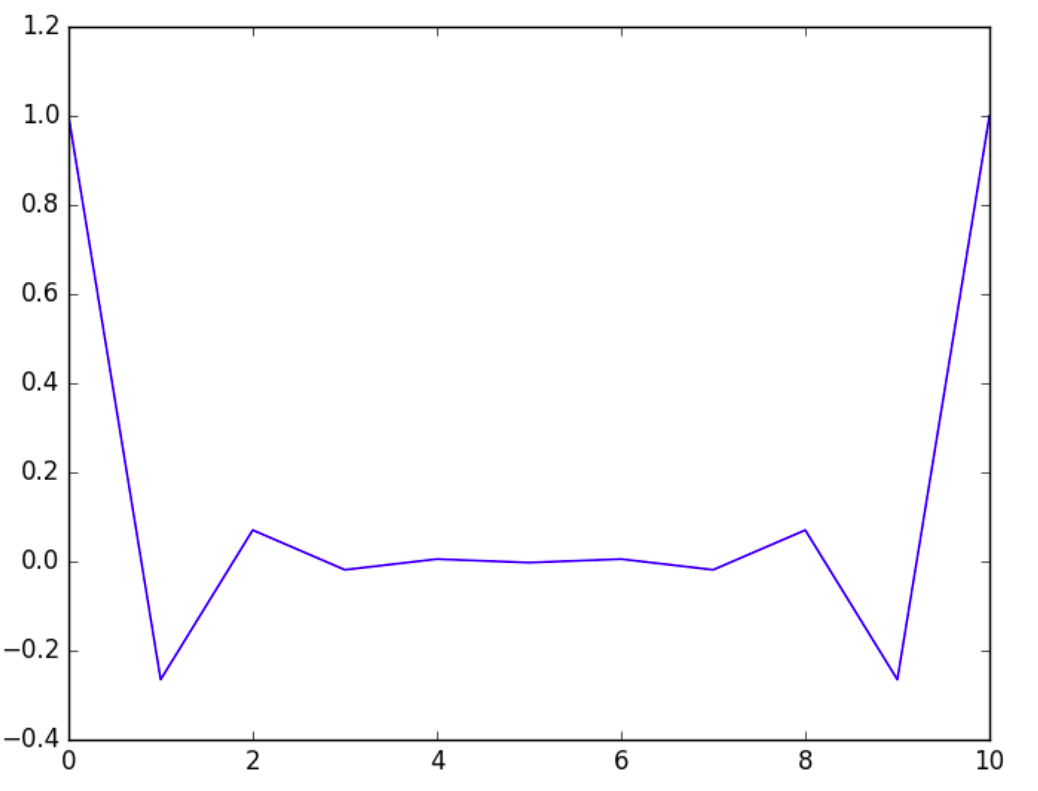
\includegraphics[width=\textwidth]{png/fenics_simpleK.png}
\end{frame}

\begin{frame}
\frametitle{Is the best approximation the best approximation?}
\begin{itemize}
\item The finite element method actually find the best approximation (in the inner
product defined by our weak form)
\item Clearly, we saw \emph{un-physical oscillations} 
\item This illustrates that the best approximation may be treacherous 
\item To guarantee oscillation-free solutions we would need monotom schemes 
or schemes that conserve special properties 
\item In this case it is natural to employ more advanced (mixed) schemes
for the Darcy problem
\end{itemize}
\end{frame}


\end{document}
